\documentclass{BHCexam}

%\usepackage[colorlinks,linkcolor=black]{hyperref}
\usepackage{makecell}%表格高度设置
\begin{document}
\biaoti{三角函数性质整理}
\fubiaoti{}
\maketitle
\setcounter{tocdepth}{2}
\tableofcontents
\newpage 
\section{基本性质}
\subsection{任意角的三角函数}
\subsubsection{任意角的概念}
\begin{enumerate}[1)]
\item 以$x$轴正方向为角度的起始边,把终边按逆时针方向旋转所成的角叫做\CJKunderdot{正角};按顺时针旋转的角叫做\CJKunderdot{负角}, 没有旋转所成的角叫\CJKunderdot{零角};
\item 终边相同的角:所有与$ \alpha $终边相同的角连同$ \alpha $在内可以构建一个集合$ S=\left\{\beta \left|\beta =\alpha+k\bm{\cdot}360^{\circ}\right.,k\inZ\right\} $.
\end{enumerate}
\subsubsection{弧度制}
把长度等于半径长的弧所对的圆心角叫做$ 1 $弧度的角,用符号$ rad $表示,读作弧度.\par
一般的,正角的弧度是正数,负角的弧度是负数,零角的弧度是$ 0. $如果半径为$ r $的圆的圆心角$ \alpha $所对的弧的长为$ l $,那么角$ \alpha $的弧度数的绝对值是:\[\abs{\alpha}=\dfrac{l}{r}.\]
角度与弧度对应关系:
$$\begin{array}{ll}
360^{\circ}=2\pi\  rad,&180^{\circ}=\pi\  rad;\\
1^{\circ}=\dfrac{\pi}{180}rad&1\ rad=\dfrac{180^{\circ}}{\pi}\approx57.30^{\circ}
\end{array}$$
\[
\begin{array}{|c*{11}{|c}|}
\hline
\text{度}&0^{\circ}& 30^{\circ}& 45^{\circ}& 60^{\circ}& 90^{\circ}& 120^{\circ}& 135^{\circ}&150^{\circ}&180^{\circ}&270^{\circ}&360^{\circ}\\\hline
\text{弧度}&0&\Gape[6pt]{\dfrac{\pi}{6}}&\dfrac{\pi}{4}&\dfrac{\pi}{4}&\dfrac{\pi}{2}&\dfrac{2\pi}{3}&\dfrac{3\pi}{2}&\dfrac{5\pi}{6}&\pi&\dfrac{3\pi}{2}&2\pi\\\hline
\end{array}
\]
\subsubsection{任意角的三角函数}
$ P(x,y) $是角$ \alpha $终边上异于原点的一点,$ \abs{OP} =r=\sqrt{x^2+y^2}$,则\[\sin\alpha=\dfrac{y}{r},\cos\alpha=\dfrac{x}{r},\tan\alpha=\dfrac{y}{x}.\]
其中$ x,y $都是带符号数,所以可以根据各象限内$ x,y $的正负性得到三角函数的符号规律:一 全正,二正弦,三两切(余切高考不涉及),四余弦.\par 

\subsubsection{同角三角函数关系}
两个重要的三角函数关系式:
\ding{192} $\sin^2\alpha+\cos^2\alpha=1;$\qquad
\ding{193} $ \tan\alpha=\dfrac{\sin\alpha}{\cos\alpha}.$
\subsubsection{诱导公式}

\begin{center}
\begin{tikzpicture}
\tikzmath{
\a =sqrt(3)/2;
\b =1/2;
\c =-\b;
}
\coordinate[label=below right:\footnotesize $O$](O) at(0,0);
\draw (0,0) circle (1cm);
\draw[->,>=latex] (-1.4,0)--(1.4,0)node[below](x){$x$};
\draw[->,>=latex] (0,-1.4)--(0,1.4)node[right](y){$y$};
\coordinate[label= right:\tiny $M$] (M) at(30:1);
\draw (0,0)--(30:1.4);
\draw[densely dashed] (30:1)|-(0.5,0);
\draw[densely dashed] (30:1)-|(0,0);
\coordinate[label=below:\tiny $M'$](M1)at(\a ,0);
\draw (0.3,0) arc(0:30:0.3);
\node[right](a) at (16:0.4) {\footnotesize $ \alpha$};
\coordinate[label=left:\tiny $N$] (N) at(120:1);
\coordinate[label=below:\tiny $N'$](N1)at(\c ,0);
%\coordinate[label=left:$N''$](M2)at(0 ,\a);
\draw (0,0)--(120:1.4);
\draw[densely dashed] (120:1)|-(0,0);
\draw[densely dashed] (120:1)-|(0,0);
\draw (0.4,0) arc(0:120:0.4);
\node[above](b) at (110:0.4) {\footnotesize$ \beta$};
\draw[rotate=30] (0,0) rectangle +(0.2,0.2);
\end{tikzpicture}
\end{center}

如上图所示,当$\beta=\dfrac{\pi}{2}+\alpha\text{时}, \triangle OMM' $和$ \triangle ONN' $全等,根据三角函数定义,可以得到:\[\cos\beta=\dfrac{ON'}{ON}=-\dfrac{MM'}{OM}=-\sin\alpha\]
即:\[\cos(\dfrac{\pi}{2}+\alpha)=-\sin\alpha \]
以此类推,可得:
$$ \sin\left(\dfrac{k\pi}{2}\pm\alpha\right)=\Bigg\{\begin{aligned}
&\pm \sin(\alpha)&k\text{为偶数},\\
&\pm \cos(\alpha)&k\text{为奇数}.
\end{aligned}~{(\kaishu \text{奇变偶不变,符号看象限})} $$
{\kaishu 此公式为自创精简写法,分析如下:当$ k $为奇数时,正(余)弦仍对应正(余)弦,当$ k $为偶数时,正(余)弦对应余(正)弦,右侧的正负号根据$ \dfrac{k\pi}{2}\pm\alpha $所在象限的正(余)弦值决定.}

\subsection{函数图象}
\subsubsection{正弦函数图象}
\begin{center}
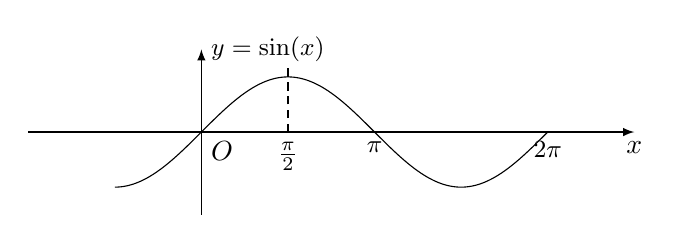
\begin{tikzpicture}[scale=0.7]
\coordinate[label=below right:$O$] (O) at(0,0);
\coordinate[label=below :\small$\pi$] (t1) at(pi,0);
\coordinate[label=below :\small$2\pi$] (t2) at(2*pi,0);
\draw[->,>=latex](-pi,0)--(2.5*pi,0)node[below](x) {$x$};
\draw[->,>=latex](0,-1.5)--(0,1.5)node[right](y) {\small $y=\sin(x)$};
\draw [domain=-pi/2:2*pi,samples=1000] plot(\x,{sin(\x r)});
\draw[densely dashed](pi/2,0)node[below](pi){$\frac{\pi}{2}$}--++(0,1.2);
\end{tikzpicture}
\end{center}
\begin{enumerate}[(1)]
\item 定义域:$x\inR$;\quad 值域:$ \left[-1,1\right] $ ;\quad 奇偶性:奇函数;
\item 对称轴:$ x=k\pi+\dfrac{\pi}{2}\left(k\inZ\right) $;\quad 对称中心:$\left(k\pi,0\right)\left(k\inZ\right)$;\quad 最小正周期:$ T=2\pi  $;
\item 单调区间:\begin{enumerate}[(i)]
\item 单调递增区间:$ \left[2k\pi-\dfrac{\pi}{2},2k\pi+\dfrac{\pi}{2}\right]\left(k\inZ\right) $;
\item 单调递减区间:$ \left[2k\pi+\dfrac{\pi}{2},2k\pi+\dfrac{3\pi}{2}\right] \left(k\inZ\right)$.
\end{enumerate}
\end{enumerate}
\subsubsection{余弦函数图象}
\begin{center}
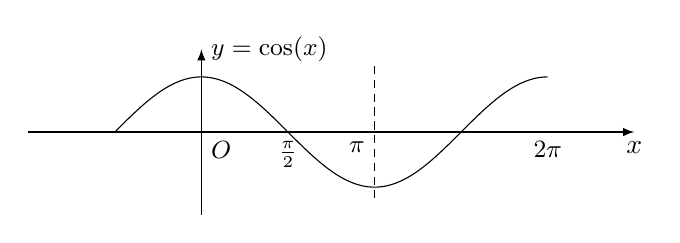
\begin{tikzpicture}[scale=0.7]
\coordinate[label=below right:\small$O$] (O) at(0,0);
\coordinate[label=below :\small $\frac{\pi}{2}$] (t1) at(pi/2,0);
\coordinate[label=below :\small $2\pi$] (t2) at(2*pi,0);
\draw[->,>=latex](-pi,0)--(2.5*pi,0)node[below](x) {$x$};
\draw[->,>=latex](0,-1.5)--(0,1.5)node[right](y) {\small $y=\cos(x)$};
\draw [domain=-pi/2:2*pi,samples=1000] plot(\x,{cos(\x r)});
\draw[densely dashed](pi,1.2)--++(0,-1.2)node[below left](pi){\small $\pi$}--++(0,-1.2);
\end{tikzpicture}
\end{center}
\begin{enumerate}[(1)]
\item 定义域:$x\inR$;\quad 值域:$ \left[-1,1\right] $;\quad 奇偶性:偶函数;
\item 对称轴:$ x=k\pi \left(k\inZ\right) $;\quad 对称中心:$\left(k\pi+\dfrac{\pi}{2},0\right)\left(k\inZ\right)$;\quad 最小正周期:$ T=2\pi  $;
\item 单调区间:\begin{enumerate}[(i)]
\item 单调递增区间:$ \left[2k\pi-\pi,2k\pi\right] \left(k\inZ\right)$;
\item 单调递减区间:$ \left[2k\pi,2k\pi+\pi\right]\left(k\inZ\right) $.
\end{enumerate}
\end{enumerate}
\subsubsection{正切函数图象}
\begin{center}
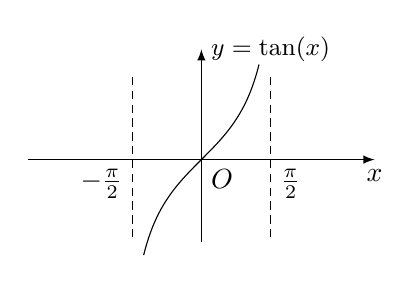
\begin{tikzpicture}[scale=0.7]
\coordinate[label=below right:$O$] (O) at(0,0);
%\coordinate[label=below :$\dfrac{\pi}{2}$] (t1) at(pi/2,0);
%\coordinate[label=below :$2\pi$] (t2) at(2*pi,0);
\draw[->,>=latex](-pi,0)--(pi,0)node[below](x) {$x$};
\draw[->,>=latex](0,-1.5)--(0,2)node[right](y) {\small $y=\tan(x)$};
\draw [domain=-pi/3:1/3*pi,samples=1000] plot(\x,{tan(\x r)});
\draw[densely dashed](2*pi/5,1.5)--++(0,-1.5)node[below right](pi){$\frac{\pi}{2}$}--++(0,-1.5);
\draw[densely dashed](-2*pi/5,1.5)--++(0,-1.5)node[below left](pi){$-\frac{\pi}{2}$}--++(0,-1.5);
\end{tikzpicture}
\end{center}
\begin{enumerate}[(1)]
\item 定义域:$\left\{x\left|x\ne k\pi+\dfrac{\pi}{2}\right.\right\}\left(k\inZ\right)$;\quad 值域:$ \mathbf{R} $;\quad 奇偶性:奇函数;
\item 对称中心:$\left(\dfrac{k\pi}{2},0\right)\left(k\inZ\right)$;\quad 最小正周期:$ T=\pi  $;
\item 单调区间:单调递增区间:$ \left(k\pi-\dfrac{\pi}{2},k\pi+\dfrac{\pi}{2}\right) \left(k\inZ\right)$;
\end{enumerate}
\subsection{$y=A\sin\left(\omega x+\varphi\right)$}
\subsubsection{$y=A\sin\left(\omega x+\varphi\right)$图象}
\begin{enumerate}[1)]
\item 用“五点法”作图:设$ z=\omega x+\varphi $,由$ z $取$ 0,\dfrac{\pi}{2},\pi,\dfrac{3\pi}{2},2\pi $来求出相应的$ x $,通过描点连线的方法画出图象.\par
{\kaishu {\heiti (注:}此处使用的$ z=\omega x+\varphi $的方法同样可以应用于求单调区间、最值等问题)}
\item 由函数$y=\sin(x)$的图象经过变换得到$y=A\sin\left(\omega x+\varphi\right)$的图象,有两种主要的途径:“先平移后伸缩”和“先伸缩后平移”
\begin{enumerate}[i)]
\item 先平移后伸缩\begin{equation*}
\begin{aligned}
y=\sin x&\xrightarrow[\text{平移}\abs{\varphi}\text{个单位}]{\text{向左}(\varphi>0)\text{或向右}(\varphi<0)}y=\sin\left(x+\varphi\right)\\
&\xrightarrow[\text{纵坐标不变}]{\text{横坐标变为原来的}\tfrac{1}{\omega}}y=\sin\left(\omega x+\varphi\right)\\
&\xrightarrow[\text{横坐标不变}]{\text{纵坐标变为原来的}A\text{倍}}y=A\sin\left(\omega x+\varphi\right)
\end{aligned}
\end{equation*}
\item 先伸缩后平移
\begin{equation*}
\begin{aligned}
y=\sin x&\xrightarrow[\text{纵坐标不变}]{\text{横坐标变为原来的}\tfrac{1}{\omega}}y=\sin\omega x\\
&\xrightarrow[\text{平移}\abs{\tfrac{\varphi}{\omega}}\text{个单位}]{\text{向左}(\varphi>0)\text{或向右}(\varphi<0)}y=\sin\left(\omega x+\varphi\right)\\&\xrightarrow[\text{横坐标不变}]{\text{纵坐标变为原来的}A\text{倍}}y=A\sin\left(\omega x+\varphi\right)
\end{aligned}
\end{equation*}
\end{enumerate}
\item 由图象求函数$y=A\sin\left(\omega x+\varphi\right)$的解析式一般步骤:
\begin{enumerate}[i)]
\item 由函数的最值确定$ A $的取值;
\item 由函数的周期确定$ \omega $的值, 周期:$ T=\dfrac{2\pi}{\abs{\omega}} $;
\item 由函数图象最高点(最低点)的坐标得到关于$ \varphi $的方程,再由$ \varphi $的范围求$ \varphi $的值.
\end{enumerate}

\item 最值:当$ x $没有范围要求时,$  A $和$ -A $分别为最大值和最小值;当$ x $有范围时,切忌将范围两端分别代入得到所谓取值范围.
\end{enumerate}
\subsubsection{$y=A\sin\left(\omega x+\varphi\right)$的单调区间问题}
\begin{enumerate}[1)]
\item 对于选择填空题,可以直接作图得到单调区间(不推荐);
\item 通用流程:\begin{enumerate}[1)]
\item 确定$ \omega $为正,若为负,则用诱导公式转化为正;
\item 确定$ A $为正,若为负,去掉负号反向取值(求$\nearrow$改成求$ \searrow $,求$ \searrow $改成求$ \nearrow $.)
\item 令$ t=\omega x+\varphi $,得到$ y=\sin t $,根据$ y=\sin t $增区间和减区间得到$ \omega x+\varphi $的范围,进而得到$ x $的取值范围.
\end{enumerate}
\end{enumerate}
\subsubsection{$y=A\sin\left(\omega x+\varphi\right)$在给定区间最值问题}\label{123}
对于给定区间$ x\in\left[x_1,x_2\right] $,有:
\begin{enumerate}
\item 设$ t=\omega x+\varphi $;
\item 将$ x $的取值代入$ \omega x+\varphi $中计算$ t$的取值范围;
\item 根据$ y=\sin t $的图象(标准图象)得到$ y $的最值及此时$ x $的取值$ x_0 $.
\end{enumerate}
\subsection{三角恒等变换}
\subsubsection{和差公式}
如下图,在半径为$ 1 $的圆内,构建向量$ \vv{OA},~\vv{OB} $.
\begin{center}
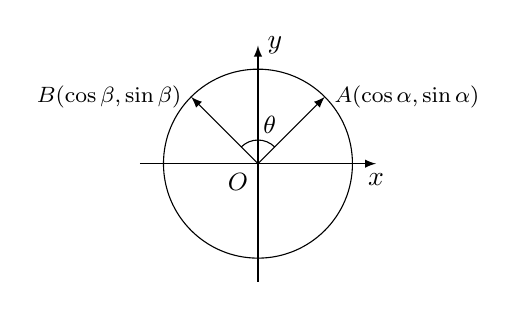
\begin{tikzpicture}
\coordinate[label=below left:\small $O$](O) at(0,0);
\draw (0,0) circle (1.2cm);
\draw[->,>=latex] (-1.5,0)--(1.5,0)node[below](x) {$x$};
\draw[->,>=latex] (0,-1.5)--(0,1.5)node[right](y) {$y$};
\draw[->,>=latex](0,0)--(45:1.2) node[right](A){\footnotesize $A(\cos\alpha,\sin\alpha)$};
\draw[->,>=latex](0,0)--(135:1.2) node[left](B){\footnotesize $B(\cos\beta,\sin\beta)$};
\draw[rotate=45] (0.3,0) arc(0:90:0.3);
\coordinate[label=\small$\theta$](t) at(60:0.3);
\end{tikzpicture}
\end{center}
根据向量夹角公式$ \cos\theta=\displaystyle\frac{\vv{OA}\bm{\cdot}\vv{OB}}{\abs{\vv{OA}}\abs{\vv{OB}}} $,将$ \vv{OA}=(\cos\alpha,\sin\alpha),\vv{OB}=(\cos\beta,\sin\beta) $代入解得:\[\cos\theta=\cos\left(\beta-\alpha\right)=\cos\alpha\cos\beta+\sin\alpha\sin\beta\]
分别令$ \alpha=-\alpha, ~\alpha=\dfrac{\pi}{2}\pm\alpha$,~由诱导公式可得:
\[\cos\left(\alpha+\beta\right)=\cos\alpha\cos\beta-\sin\alpha\sin\beta\]
\[\sin\left(\alpha+\beta\right)=\sin\alpha\cos\beta+\cos\alpha\sin\beta\]
\[\sin\left(\alpha-\beta\right)=\sin\alpha\cos\beta-\cos\alpha\sin\beta\]
在$ \sin(\alpha+\beta)\text{和} \cos(\alpha+\beta)$中令$ \beta=\alpha $得到倍角公式:

\[\begin{aligned}
\sin2\alpha=&2\sin\alpha\cos\alpha\\
\cos2\alpha=&\cos^2\alpha-\sin^2\alpha\\
=&2\cos^2\alpha-1\\
=&1-2\sin^2\alpha.
\end{aligned}\]
\subsubsection{半角公式}
\begin{enumerate}[1)]
\item $\sin ^2x=\dfrac{1-\cos2x}{2}$
\item $\cos ^2x=\dfrac{1+\cos 2x}{2}$
\end{enumerate}
\subsubsection{辅助角公式}
对于$ y=a\sin x+b\cos x $类型的三角函数的性质需要先化简为$y=A\sin\left(\omega x+\varphi\right)$形式,所以引入角$ \varphi $使其正余弦和$ a,b $对应,根据$ \sin^2\varphi+\cos^2\varphi=1 $可得到如下形式:
\begin{equation*}\begin{aligned}
a\sin x+b\cos x=&\sqrt{a^2+b^2}\left(\dfrac{a}{\sqrt{a^2+b^2}}\sin x+\dfrac{b}{\sqrt{a^2+b^2}}\cos x\right)\\
=&\sqrt{a^2+b^2}\left(\sin x\cos \varphi+\cos x\sin\varphi\right)\\
=&\sqrt{a^2+b^2}\sin\left(x+\varphi\right)~\left(\tan\varphi=\dfrac{b}{a}\right)
\end{aligned}
\end{equation*}
由此公式可看出$ \sin\varphi=\dfrac{b}{\sqrt{a^2+b^2}},~\cos\varphi=\dfrac{a}{\sqrt{a^2+b^2}} $;\\
可根据实际情况令$  \cos\varphi=\dfrac{b}{\sqrt{a^2+b^2}},~\sin\varphi=\dfrac{a}{\sqrt{a^2+b^2}} $得到辅助角公式的余弦形式.
\subsection{三角函数化简求值问题}
\subsubsection{化简“三看”原则}
\begin{enumerate}[(1)]
\item 一看“角”,~通过看角之间的差别与联系(比如出现了$ \alpha $和$ 2\alpha $就会使用倍角公式),~正确的使用公式;
\item 二看“函数名称”,~看函数名称之间的差异,从而确定使用的公式,例如:切化弦,正余弦互化;
\item 三看“结构特征”,~分析结构特征可以帮助我们找到变形的方向,常见的有“遇到分式要通分”等.
\end{enumerate}
\subsubsection{求最值问题}\begin{enumerate}[(1)]
\item $ y=a\sin x+b\cos x=\sqrt{a^2+b^2}\sin\left(\omega x+\varphi\right) $,~ 利用有界性处理(参考\ref{123});
\item $ y=a\sin^2x+b\sin x\cos x+\cos^2x \xrightarrow{\text{降次,整理}}y=A\sin 2x+B\cos2x+C=\sqrt{A^2+B^2}\sin(2x+\varphi)+C$,~其中$ \tan\varphi=\dfrac{B}{A} .$再利用有界性;
\item $ y=a\sin^2x+b\sin x+c \text{或}y=a\cos^2x+b\cos x+c(a\ne0)$,~通过$ t=\sin x $或$ t=\cos x $转化为求关于$ t $的二次函数在区间$ \left[-1,1\right]$上的最值问题;
\item $y=a\left(\sin x\pm\cos x\right)+b\sin x\bm{\cdot}\cos x $,可令$ t=\sin x\pm\cos x $,则$ \sin x\bm{\cdot}\cos x=\pm\dfrac{t^2-1}{2} $,把三角问题转化为代数问题解决;
\item $ y=\dfrac{a\sin x+c}{b\sin x+d} $或$ y=\dfrac{a\cos x+c}{b\cos x+d} $可转化为只有分母含有$ \sin x  $或$ \cos x $的函数式,还可以转化为$ \sin x=f(y) $或$ \cos x=f(y) $的形式,由正、余弦函数的有界性求解.
\item $y=\dfrac{a\sin x+c}{b\cos x+d}\left(\text{或}y=\dfrac{a\cos x+c}{b\sin x+d}\right)$,其中$ ab\ne0 $,先化为$ y=\dfrac{a}{b}\times\dfrac{\sin x+\dfrac{c}{a}}{\cos x+\dfrac{d}{b}} \text{或}y=\dfrac{a}{b}\times\dfrac{\cos x+\dfrac{c}{a}}{\sin x+\dfrac{d}{b}} $,则转化为求圆上的动点与定点连线斜率的最值问题.
\end{enumerate}
\section{解三角形}
\subsection{正弦、余弦定理}
\subsubsection{正弦定理}
在三角形$\triangle ABC$中,角$ A,B,C $所对的边为$ a,b,c $,~有$$ \dfrac{a}{\sin A}=\dfrac{b}{\sin B}=\dfrac{c}{\sin C}=2R~(R\text{\kaishu 为外接圆半径,高考没考过半径})$$
\begin{proof}
此处以直角三角形为例.如下图,设角$ A,B,C $所对的边分别为$ a,b,c $,则有:
\begin{center}
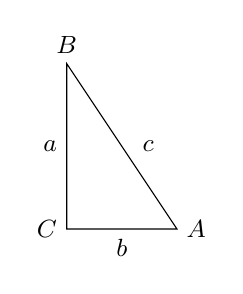
\begin{tikzpicture}[scale=0.7]
\coordinate[label=left:\small$C$](C) at(0,0);
\coordinate [label=above:\small $B$](B)at (0,3);
\coordinate [label=right:\small $A$](A)at (2,0);
\coordinate[label=right:\small$c$](c) at(1.2,1.5);
\coordinate [label=below:\small $b$](b)at (1,0);
\coordinate [label=left:\small $a$](a)at (0,1.5);
\draw(A)--(B)--(C)--cycle;
\end{tikzpicture}
\end{center}
由直角三角形对应的三角函数定义知$$  \sin A=\dfrac{a}{c},~\sin B=\dfrac{b}{c},~\sin C=\dfrac{c}{c}=1$$
即:  $$\dfrac{a}{\sin A}=\dfrac{b}{\sin B}=\dfrac{c}{\sin C}=c=2R$$
非直角三角形推导过程类似,通过构建高线得到直角三角形.
\end{proof}
正弦定理的主要作用是方程和分式中的边角互化.其原则为关于边,或是角的正弦值是否具备齐次的特征.如果齐次则可直接进行边化角或是角化边,否则不可行.
\subsubsection{余弦定理}
\begin{itemize}
\item $ c^2=a^2+b^2-2ab\cos C ~\text{或}\cos C=\dfrac{a^2+b^2-c^2}{2ab}$
\item 另外两个一样,我不想写了.
\end{itemize}
\begin{proof}
在三角形$\triangle ABC$中,角$ A,B,C $所对的边分别为$ a,b,c $,如图所示,构建向量$ \vv{a},\vv{b},\vv{c} $.
\begin{center}
\begin{tikzpicture}[scale=0.7]
\tikzmath{\c =3*sin(60);
}
\coordinate[label=left:\small$A$](A) at(0,0);
\coordinate[label=right:\small$B$](B) at(3,0);
\coordinate[label=above:\small$C$](C) at(1.5,\c);
\draw[->,>=latex](A)--(B)node[midway,below]{$\vv{c}$};
\draw[->,>=latex](C)--(A)node[midway,above left]{$\vv{b}$};
\draw[->,>=latex](C)--(B)node[midway,above right]{$\vv{a}$};
\end{tikzpicture}
\end{center}
由向量减法知:$ \vv{a}-\vv{b}=\vv{c} $两边平方得到$$ \left(\vv{a}-\vv{b}\right)^2=\vv{c}^2 $$
展开得到$$ a^2+b^2-2ab\cos C=c^2 $$\text{\kaishu(这里直接将向量模长写成边长了,代码太多了$ \ldots $)}
\end{proof}
\subsection{解三角形常用结论}
\begin{enumerate}[1)]
\item $A+B+C=\pi$;\quad $\sin\left(A+C\right)=\sin B$;\quad $\cos\left(A+C\right)=-\cos B$.
\item $S=\dfrac{1}{2}ab\sin C=\dfrac{1}{2}ac\sin B=\dfrac{1}{2}bc\sin A$;
\item $ \sin^2A+\sin^2B-\sin A\sin B=\sin^2C \Leftrightarrow a^2+b^2-ab=c^2$
\item $b\cos C+c\cos B=a\Rightarrow \sin B\cos C+\sin C\cos B=\sin A$~(恒等式)
\item $A>B>C\Leftrightarrow a>b>c\Leftrightarrow \sin A>\sin B>\sin C\Leftrightarrow \cos A<\cos B<\cos C$
\end{enumerate}

\subsection{解三角形问题主要思路}
\subsubsection{公式适用类型}
\begin{enumerate}[1)]
\item 已知两角一边,用正弦定理,有解时,只有一解;
\item 已知两边及一边对角,用正弦定理,有解的情况(设已知$ a,b $和角$ A $):\begin{enumerate}[a)]
\item $ A $为锐角,当$ a<b\sin A $时无解;若$ A $为钝角,当$ a=b,a<b $时均无解;
\item 若为求第三边问题,也可以通过余弦定理构造一元二次方程求解.
\end{enumerate}
\item 已知三边,用余弦定理,有解时,只有一解;
\item 已知两边及夹角,用余弦定理,必有一解.
\end{enumerate}
\subsubsection{解三角形最值问题}
\begin{enumerate}[(1)]
\item 利用正弦定理将边转化为角,通过三角恒等变换转化为$ y=A\sin\left(\omega x+\varphi\right) $,在满足内角和为$ \pi $的范围内求最值.
\item 对于某些乘法的最值(例如面积最大值)利用余弦定理转化为边的形式,利用基本不等式$ a^2+b^2\ge2ab $求最值.
\end{enumerate}
\section{练习}
\begin{questions}


\qs 已知$\sin 2\alpha=\dfrac{2}{3}$,则$\cos^2\left(\alpha+\dfrac{\pi}{4}\right)=$\xx
\onech{$\dfrac{1}{6}$}{$\dfrac{1}{3}$}{$\dfrac{1}{2}$}{$\dfrac{2}{3}$}
\qs 若$ \sin \left(\dfrac{\pi}{6}-\alpha\right)=\dfrac{1}{3},\  $则$ \cos \left(\dfrac{2\pi}{3}+2\alpha\right)= $\xx
\onech{$ -\dfrac{7}{9}$}{$ -\dfrac{1}{3}$}{$ \dfrac{1}{3}$}{$ \dfrac{7}{9}$}
\qs 若$ \tan \theta+\dfrac{1}{\tan \theta} =4,\ $则$ \sin 2\theta =$\xx
\onech{$ \dfrac{1}{5}$}{$ \dfrac{1}{4}$}{$ \dfrac{1}{3}$}{$ \dfrac{1}{2}$}


\question 设$\alpha \in \left(0,\dfrac{\pi}{2}\right),\beta \in \left(0,\dfrac{\pi}{2}\right)$,且$\tan \alpha =\dfrac{1+\sin \beta}{\cos \beta}$,则\xx
\twoch{$3\alpha-\beta=\dfrac{\pi}{2}$}{$3\alpha+\beta=\dfrac{\pi}{2}$}{$2\alpha-\beta=\dfrac{\pi}{2}$}{$2\alpha+\beta=\dfrac{\pi}{2}$}
\question 函数$f(x)=\cos 2x+6\cos \left(\dfrac{\pi}{2}-x\right)$的最大值为\xx
\onech{4}{5}{6}{7}

\qs 将函数$ y=\sin\left(2x+\dfrac{\pi}{3}\right) $图象上的点$ P\left(\dfrac{\pi}{4},t\right) $向左平移$ s\ (s>0) $个单位长度得到点$ P' $.若$ P' $位于函数 $ y=\sin 2x $的图象上,则\xx
\twoch{$ t=\dfrac{1}{2},\ s\text{的最小值为}\dfrac{\pi}{6} $}{$ t=\dfrac{\sqrt{3}}{2},\ s\text{的最小值为}\dfrac{\pi}{6} $}{$ t=\dfrac{1}{2},\ s\text{的最小值为}\dfrac{\pi}{3} $}{$ t=\dfrac{\sqrt{3}}{2},\ s\text{的最小值为}\dfrac{\pi}{3} $}
\question 已知函数$f(x)=\sin(\omega x+\varphi)\ \left(\omega>0,\ \abs{\varphi}\le \dfrac{\pi}{2}\right),x=-\dfrac{\pi}{4}$为$f(x)$的零点,$x=\dfrac{\pi}{4}$为$y=f(x)$图象的对称轴,且$f(x)$在$\left(\dfrac{\pi}{18},\dfrac{5\pi}{36}\right)$单调,则$\omega$的最大值为\xx
\onech{11}{9}{7}{5}
\qs 已知$ \omega>0,\  $函数$f(x)=\sin \left(\omega x+\dfrac{\pi}{4}\right)$在$\left(\dfrac{\pi}{2},\pi\right)  $上单调递减,则$ \omega $的取值范围是\xx
\onech{$ \left[\dfrac{1}{2},\dfrac{5}{4}\right] $}{$ \left[\dfrac{1}{2},\dfrac{3}{4}\right] $}{$ \left(0,\dfrac{1}{2}\right] $}{$ \left(0,2\right] $}
\qs 已知$ \omega>0,\ 0<\varphi <\pi,\  $直线$ x=\dfrac{\pi}{4} $和$ x=\dfrac{5\pi}{4} $是函数$f(x)=\sin (\omega x+\varphi)$的图象的两条相邻对称轴,则$ \varphi= $\xx
\onech{$ \dfrac{\pi}{4} $}{$ \dfrac{\pi}{3} $}{$ \dfrac{\pi}{2} $}{$ \dfrac{3\pi}{4} $}

\qs 将函数$f(x)=\sin (2x+\theta)\left(-\dfrac{\pi}{2}<\theta<\dfrac{\pi}{2}\right)$的图象向右平移$ \varphi(\varphi>0) $个单位长度后得到函数$g(x)$的图象,若$f(x),\ g(x)$的图象都经过点$ P\left(0,\dfrac{\sqrt{3}}{2}\right) $,\ 则$ \varphi $的值可以是\xx
\onech{$ \dfrac{5\pi}{3}$}{$ \dfrac{5\pi}{6}$}{$ \dfrac{\pi}{2}$}{$ \dfrac{\pi}{6}$}
\qs 已知函数$f(x)=2\sin \left(\omega x+\varphi\right),\ x \inR$,\ 其中$ \omega>0,\ -\pi <\varphi\le \pi ,\  $若$f(x)$的最小正周期为$ 6\pi  $,且当$ x=\dfrac{\pi}{2} $时,$f(x)$取得最大值,则\xx
\twoch{$f(x)$在区间$ \left[-2\pi,0\right] $上是增函数}{$f(x)$在区间$ \left[-3\pi,-\pi \right] $上是增函数}{$f(x)$在区间$ \left[3\pi,5\pi \right] $上是减函数}{$f(x)$在区间$ \left[4\pi,6\pi \right] $上是减函数}

\qs 已知函数$f(x)=\sin (\omega x +\varphi)+\cos (\omega x+\varphi)\ \left(\omega>0,\ \left|\varphi\right|<\dfrac{\pi}{2}\right)$的最小正周期为$ \pi , $且$ f(-x)=f(x),\  $则\xx
\twoch{$ f(x) $在$ \left(0,\dfrac{\pi}{2}\right) $上单调递减}{$ f(x) $在$ \left(\dfrac{\pi}{4},\dfrac{3\pi}{4}\right) $上单调递减}{$ f(x) $在$ \left(0,\dfrac{\pi}{2}\right) $上单调递增}{$ f(x) $在$ \left(\dfrac{\pi}{4},\dfrac{3\pi}{4}\right) $上单调递增}
\qs 已知函数$f(x)=\Bigg\{\begin{aligned}
\sin(x+\alpha),x\le 0\\\cos (x+\alpha),x>0
\end{aligned}$则“$ \alpha=\dfrac{\pi}{4} $”是“函数$f(x)$是偶函数”的\xx
\twoch{充分不必要条件}{必要不充分条件}{充分必要条件}{既不充分也不必要条件}
\qs 已知函数$f(x)=\Bigg\{\begin{aligned}
\sin(x+a),x\le 0\\\cos (x+b),x>0
\end{aligned}$是偶函数,则下列结论可能成立的是\xx

 \twoch{$ a=\dfrac{\pi}{4},b=-\dfrac{\pi}{4}$}{$ a=\dfrac{2\pi}{3},b=\dfrac{\pi}{6}$}{$a=\dfrac{\pi}{3},b=\dfrac{\pi}{6} $}{$ a=\dfrac{5\pi}{6},b=\dfrac{2\pi}{3}$}



\qs 在$\triangle ABC$中,$ \angle A=\dfrac{\pi}{3},\ BC=3 $,则$ \triangle ABC $的周长为\xx
\twoch{$ 4\sqrt{3}\sin \left(B+\dfrac{\pi}{3}\right)+3$}{$4\sqrt{3}\sin \left(B+\dfrac{\pi}{6}\right)+3 $}{$6\sin \left(B+\dfrac{\pi}{3}\right)+3 $}{$ 6\sin \left(B+\dfrac{\pi}{6}\right)+3$}

\qs $\triangle ABC$的内角$ A,B,C $所对的边分别为$ a,b,c $.若$ a\sin A\sin B+b\cos^2A=\sqrt{2}a,\  $则$ \dfrac{b}{a}=$\xx
\onech{$ 2\sqrt{3}$}{$ 2\sqrt{2}$}{$ \sqrt{3}$}{$ \sqrt{2}$}
\qs 在$ \triangle ABC $中,若$ \sin ^2A+\sin^2 B<\sin ^2C $,则$ \triangle ABC $的形状是\xx
\twoch{钝角三角形}{直角三角形}{锐角三角形}{不能确定}
\qs 已知锐角$\triangle ABC$的内角$A,B,C$的对边分别为$a,b,c$,$23\cos^2A+\cos 2A=0$,$a=7$,$c=6$,则$b=$\xx
\onech{10}{9}{8}{5}
\qs 已知函数$f(x)=\sin \left(\omega x-\dfrac{\pi}{3}\right)$,\ 点$ A(m,n) $,\ $ B(m+\pi,n) (\left|n\right|\ne 1)$都在曲线$ y=f(x) $上,且线段$ AB $与曲线$ y=f(x) $有五个公共点,则$ \omega $的值为\xx
\onech{$ 4 $}{$ 2 $}{$ \dfrac{1}{2} $}{$ \dfrac{1}{4} $}


\qs 设$\theta$为第二象限角,若$ \tan\left(\theta +\dfrac{\pi}{4}\right)=\dfrac{1}{2},\  $则$ \sin \theta+\cos \theta $=\tk.

\qs 已知$\sin \alpha=\dfrac{1}{2}+\cos \alpha,\ $且$ \alpha\in \left(0,\dfrac{\pi}{2}\right),\  $则$ \dfrac{\cos 2\alpha}{\sin \left(\alpha-\dfrac{\pi}{4}\right)} $的值为\tk.
\question 函数$f(x)=\sin \left(x+2\varphi\right)-2\sin \varphi \cos(x+\varphi)$的最大值为\tk.
\question 设当$x=\theta$时,函数$f(x)=\sin x-2\cos x$取得最大值,则$\cos \theta=$\tk.

\qs 已知函数$f(x)=2\sin \omega x\ (\omega>0)$在区间$ \left[-\dfrac{\pi}{3},\dfrac{\pi}{4}\right] $上的最小值是$ -2 $,则$ \omega $的最小值是\tk.
\qs 已知函数$f(x)=\sin (2x+\varphi)$,若$    f\left(\dfrac{\pi}{12}\right)-f\left(\dfrac{-5\pi}{12}\right)=2 $,则函数$f(x)$的单调增区间为\tk.
\qs 设函数$ f(x)=A\sin\left(\omega x+\varphi\right)\ \left(A,\omega,\varphi \text{是常数,}A>0,\omega>0\right)$.若$ f(x) $在区间$ \left[\dfrac{\pi}{6},\dfrac{\pi}{2}\right] $上具有单调性,且$f\left(\dfrac{\pi}{2}\right)=f\left(\dfrac{2\pi}{3}\right)=-f\left(\dfrac{\pi}{6}\right) $,则$ f(x) $的最小正周期是\tk.
\qs 将函数$f(x)=\sin (\omega x+\varphi)\ \left(\omega >0,-\dfrac{\pi}{2}\le \varphi<\dfrac{\pi}{2}\right)$图像上每个点的横坐标缩短为原来的一半,纵坐标不变,再向右平移$ \dfrac{\pi}{6} $个单位长度得到$ y=\sin x $的图象,则$ f\left(\dfrac{\pi}{6}\right) $\tk.
\qs 已知点$ A\left(\dfrac{\pi}{6},\dfrac{\sqrt{3}}{2}\right),\ B\left(\dfrac{\pi}{4},1\right),\ C\left(\dfrac{\pi}{2},0\right)$,若这三个点中有且仅有两个点在函数$f(x)=\sin \omega x$的图象上,则\CJKunderdot{正数}$ \omega $的最小值为\tk.

\qs 函数$y=\cos (2x+\varphi)\ (-\pi<\varphi<\pi)$的图象向右平移$\dfrac{\pi}{2}$个单位后,与函数$y=\sin (2x+\dfrac{\pi}{3})$的图象重合,则$\varphi=$\tk.
\qs 把函数$ y=\sin 2x $的图象沿$x$轴向左平移$ \dfrac{\pi}{6} $个单位,纵坐标伸长到原来的2倍(横坐标不变)后得到函数$ y=f(x) $的图象,对于函数$ y=f(x) $有以下四个判断:\\
\ding{192} 该函数的解析式为$ y=2\sin \left(2x+\dfrac{\pi}{6}\right) $;\\
\ding{193} 该函数图象关于点$ \left(\dfrac{\pi}{3},0\right) $对称;\\
\ding{194} 该函数在$ \left[0,\dfrac{\pi}{6}\right] $上是增函数;\\
\ding{195} 若函数$ y=f(x)+a $在$ \left[0,\dfrac{\pi}{2}\right] $上的最小值为$ \sqrt{3},\  $则$ a=2\sqrt{3} .$\\
其中,正确判断的序号是\tk.




\qs 在三角形$\triangle ABC$中,$ B=60^{\circ} $,$ AC=\sqrt{3} $,则$ AB+2BC $的最大值为\tk.


\qs 在三角形$\triangle ABC$中,$ a=3,b=\sqrt{6} $,$ \angle A=\dfrac{2\pi}{3} $,则$ \angle B= $\tk.

\qs 在三角形$\triangle ABC$中,若$ a=2,\ b+c=7,\ \cos B=-\dfrac{1}{4} $,则$ b= $\tk.

\qs 在三角形$\triangle ABC$中,$ a=4,b=5,c=6 $,则$ \dfrac{\sin 2A}{\sin C}=$\tk.
\qs 若$\triangle ABC$的内角满足$ \sin A+\sqrt{2}\sin B=2\sin C $,则$ \cos C $的最小值是\tk.
\question 在平面四边形$ABCD$中,$\angle A=\angle B=\angle C=75^{\circ},\ $$ BC=2,\  $则$AB$的取值范围是\tk.
\qs 在$\triangle ABC$中,$ D $为$ BC $边上的一点,$ BC=3BD,\ AD=\sqrt{2},\ \angle ADB=135^{\circ}.\  $若$ AC=\sqrt{2}AB $,则$ BD= $\tk.
\question 已知$a,\ b,\ c$分别为$\triangle ABC$三个内角$A$,\ $B$,\ $C$的对边,$a=2$,且$(2+b)(\sin A-\sin B)=(c-b)\sin C$,则$\triangle ABC$面积的最大值为\tk.
\qs 在三角形$\triangle ABC$中,$ \angle BAD=30^{\circ},\angle CAD=45^{\circ},\ AB=2,\ AC=2 $则$ \dfrac{BD}{DC}= $\tk.
\vspace{-2em}
\begin{center}
\begin{tikzpicture}[line width=0.7 pt,scale=0.7]
%\draw[help lines] (0,0) grid (4,3);
\coordinate[label=below:\small$B$](B) at (0,0);
\coordinate[label=below:\small$C$](C) at(3,0);
\coordinate [label=above:\small$A$](A) at(2,2);
\coordinate [label=below:\small$D$](D) at ($(B)!0.4!(C)$);
\draw (B)--(A)--(C)--cycle (A)--(D);
\end{tikzpicture}
\end{center} 



\qs 已知$a,b,c$分别为$\triangle ABC$内角$A,B,C$的对边,$\sin^2B=2\sin A\sin C$.
\begin{parts}
\part 若$a=b$,求$\cos B$;
\part 若$B=90^{\circ}$,且$a=\sqrt{2}$,求$\triangle ABC$的面积.
\end{parts}
\kongbai
\qs 在$ \triangle ABC $中,$ a^2+c^2=b^2+\sqrt{2}ac $.
\begin{parts}
\part 求$ \angle B $的大小;
\part 求$ \sqrt{2}\cos A+\cos C $的最大值.
\end{parts}
\newpage
\qs 已知函数$f(x)=2\sin \omega x\cos \omega x+\cos 2\omega x (\omega >0) $的最小正周期为$ \pi $.
\begin{parts}
\part 求$ \omega $的值;
\part 求$ f(x) $的单调递增区间.
\end{parts}
\kongbai
\qs 已知函数$f(x)=\sqrt{2}\sin \dfrac{x}{2}\cos \dfrac{x}{2}-\sqrt{2}\sin^2 \dfrac{x}{2}$.
\begin{parts}
\part 求$ f(x) $的最小正周期
\part 求$ f(x) $在区间$\left[-\pi,0\right]$上的最小值.
\end{parts}
\kongbai
\qs 已知函数$f(x)=\sin x-2\sqrt{3}\sin^2 \dfrac{x}{2}$.
\begin{parts}
\part 求$ f(x)  $的最小正周期;
\part 求$ f(x) $在区间$ \left[0,\dfrac{2\pi}{3}\right] $上的最小值.
\end{parts}
\kongbai
\qs $\triangle ABC$的内角$ A,B,C $的对边$ a,b,c \ $.已知$ 2\cos C(a\cos B +b \cos A)=c $.
\begin{parts}
\part 求$ C $;
\part 若$ c=\sqrt{7} $,$ \triangle ABC $的面积为$ \dfrac{3\sqrt{3}}{2} $,求$ \triangle ABC $的周长.
\end{parts}
\kongbai
\qs 如图,在三角形$\triangle ABC$中,$ \angle B=\dfrac{\pi}{3} ,\  AB=8 $,点$ D $在$ BC $边上,且$ CD=2 ,\  \cos \angle ADC=\dfrac{1}{7} $
\begin{parts}
\part 求$ \sin \angle BAD $;
\part 求$ BD,\ AC $的长.
\end{parts}
\vspace{-4em}\mbox{\hspace{1pt}}\hfill
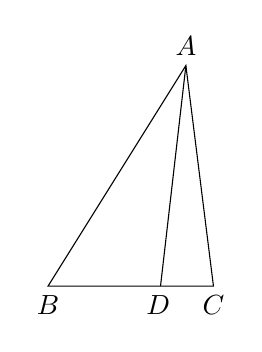
\begin{tikzpicture}[x=0.7cm, y=0.7cm]
\draw (0,0) node[below ](B){$B$}--(2,0) node[below] (D) {$D$}--(3,0)node[below] (C) {$C$}--(2.5,4) node[ above] (A) {$A$}--cycle;
\draw (2.5,4)--(D);
\end{tikzpicture}
\newpage
\qs 已知函数$f(x)=\left(2\cos^2 x-1\right)\sin 2x+\dfrac{1}{2}\cos 4x$
\begin{parts}
\part 求$ f(x) $的最小正周期及最大值;
\part 若$ \alpha \in \left(\dfrac{\pi}{2},\pi \right) $,且$ f(\alpha )=\dfrac{\sqrt{2}}{2} $,求$ \alpha $的值.
\end{parts}
\kongbai
\qs
已知函数$f(x)=4\cos x\sin \left(x+\dfrac{\pi}{6}\right)-1.$
\begin{parts}
\part 求$ f(x) $的最小正周期
\part 求$ f(x) $在区间$ \left[-\dfrac{\pi}{6},\dfrac{\pi}{4}\right] $上的最大值和最小值.
\end{parts}
\newpage
\qs 已知函数$f(x)=2\cos 2x+\sin^2 x-4\cos x$.
\begin{parts}
\part 求$ f\left(\dfrac{\pi}{3}\right) $的值;
\part 求$ f(x) $的最大值和最小值.
\end{parts}
\kongbai
\qs 在三角形$\triangle ABC$中,内角$ A,\ B,\ C,\  $对边的边长分别是$ a,\ b,\ c ,\ $已知$ c=2,C=\dfrac{\pi}{3} .$
\begin{parts}
\part 若三角形$\triangle ABC$的面积等于$\sqrt{3},\  $求$ a,b $;
\part 若$ \sin C+\sin (B-A)=2\sin 2A,\  $求$ \triangle ABC $的面积.
\end{parts}
\newpage
\qs 已知函数$f(x)=\sin^2 \omega x+2\sqrt{3}\sin \omega x\bm{\cdot}\cos \omega x-\cos^2 \omega x+\lambda$的图象关于直线$ x=\pi $对称,其中$ {\omega ,\lambda} $为常数,且$ \omega \in \left(\dfrac{1}{2},1\right). $
\begin{parts}
\part 求函数$f(x)$的最小正周期;
\part 若$ y=f(x) $的图象经过点$ \left(\dfrac{\pi}{4},0\right),\  $求函数$f(x)$的值域.
\end{parts}
\kongbai
\qs 在三角形$\triangle ABC$中,角$A,\ B,\ C,\ $所对的边长分别是$a,\ b,\ c,\ $且$ a\cos B=3,\ b\sin A=4. $
\begin{parts}
\part 求边长$ a; $
\part 若三角形$\triangle ABC$的面积$ S=10,\  $求$ \triangle ABC $的周长$ l. $
\end{parts}
\kongbai
\qs 在三角形$\triangle ABC$中,角$A,\ B,\ C,\ $所对的边长分别是$a,\ b,\ c,\ $已知$ \cos C+(\cos A-\sqrt{3}\sin A)cos B=0. $
\begin{parts}
\part 求角$ B $的大小;
\part 若$ a+c=1,\  $求$ b $的取值范围.
\end{parts}
\kongbai
\qs 在锐角三角形$\triangle ABC$中,角$A,\ B,\ C,\ $所对的边长分别是$a,\ b,\ c,$且$ \sqrt{3}a=2c\sin A $
\begin{parts}
\part 确定角$ C $的大小;
\part 若$ c=\sqrt{7},\  $且三角形$\triangle ABC$的面积为$ \dfrac{3\sqrt{3}}{2},\  $求$ a+b $的值.
\end{parts}
\kongbai
\qs 四边形$ ABCD $ 的内角$ A $与$ C $互补,$ AB=1,\ BC=3,\ CD=DA=2. $
\begin{parts}
\part 求$ C $和$ BD $;
\part 求四边形$ ABCD $的面积.
\end{parts}
\kongbai
\qs 在三角形$\triangle ABC$中,角$A,\ B,\ C,\ $所对的边长分别是$a,\ b,\ c,\ $已知$ \cos (A-C)+\cos B=1,\ a=2c, $求$ C $.
\kongbai
\qs 在三角形$\triangle ABC$中,角$A,\ B,\ C,\ $所对的边长分别是$a,\ b,\ c,\ $已知$ A=\dfrac{\pi}{4},\ b\sin \left(\dfrac{\pi}{4}+C\right)-c\sin \left(\dfrac{\pi}{4}+B\right)=a. $求证:$ B-C=\dfrac{\pi}{2}. $
\kongbai
\qs $\triangle ABC$中的内角$ A,\ B,\ C $的对边分别为$ a,\ b,\ c,\  $已知$ a=b\cos C+c\sin B $.
\begin{parts}
\part 求$ B $;
\part 若$ b=2 $,求$\triangle ABC$面积的最大值.
\end{parts}
\kongbai
\qs 在$\triangle ABC$中,内角$ A,\ B,\ C $的对边长分别为$ a,\ b,\ c $,已知$ a^2-c^2=2b $,且$ \sin B=4\cos A\sin C $,求$ b $.
\kongbai
\qs 已知函数$f(x)=-2\sin x-\cos 2x$.
\begin{parts}
\part 比较$ f(\dfrac{\pi}{4}) ,\ f(\dfrac{\pi}{6})$的大小;
\part 求函数$f(x)$的最大值.
\end{parts}
\kongbai
\qs 在锐角$\triangle ABC$中,角$ A,B,C $所对的边分别为$ a,b,c $,已知$ a=\sqrt{7},\ b=3,\ \sqrt{7}\sin B+\sin A=2\sqrt{3}.$
\begin{parts}
\part 求角$ A $的大小;
\part 求$\triangle ABC$的面积
\end{parts}
\kongbai
\qs 在三角形$\triangle ABC$中,角$ A,\ B,\ C $所对的边分别为$ a,\ b,\ c $,且$ \sin^2 A=\sin B\sin C $.
\begin{parts}
\part 若$ \angle A=\dfrac{\pi}{3},\  $求$ \angle B $的大小;
\part 若$ bc=1, \ $求$\triangle ABC$的面积的最大值.
\end{parts}
\kongbai
\qs 如图,在三角形$\triangle ABC$中,$ \angle ABC=90^{\circ} ,AB=4,BC=3,\ $点$ D $在线段$ AC $上,且$ AD=4DC $.
\begin{parts}
\part 求$ BD $的长;
\part 求$ \sin CBD $的值.
\end{parts}
\mbox{\hspace{1em}}\hfill
\begin{tikzpicture}[line width=0.7 pt,scale=0.7]
%\draw[help lines] (0,0) grid (4,3);
\coordinate[label=left:$B$](B) at (0,0);
\coordinate[label=right:$C$](C) at(3,0);
\coordinate [label=above:$A$](A) at(0,4);
\coordinate [label=right:$D$](D) at ($(A)!0.75!(C)$);
\draw (B)--(A)--(C)--cycle (B)--(D);
\end{tikzpicture}
\kongbai
\vspace{-7em}
\qs 已知函数$f(x)=\left(1+\sqrt{3}\tan x\right)\cos^2x .$
\begin{parts}
\part 若$ \alpha $是第二象限角,且$ \sin \alpha=\dfrac{1}{3} $,求$ f(\alpha) $的值;
\part 求函数$f(x)$的定义域和值域. 
\end{parts}
\newpage
\qs 在三角形$\triangle ABC$中,角$ A,\ B,\ C $所对的边分别为$ a,\ b,\ c ,\ $已知$ b^2+c^2=a^2+bc. $
\begin{parts}
\part 求$ A $的大小;
\part 如果$ \cos B=\dfrac{\sqrt{6}}{3},b=2 ,\ $求三角形$\triangle ABC$的面积.
\end{parts}
\kongbai
\qs 已知函数$f(x)=2\sin \dfrac{\pi}{6}x\cos \dfrac{\pi}{6}x,\ $过两点$ A\left(t,f(t)\right) ,\ B\left(t+1,f(t+1)\right)$的直线的斜率记为$ g(t). $
\begin{parts}
\part 求$ g(0) $的值;
\part 写出函数$ g(x) $的解析式,求$ g(t) $在$ \left[-\dfrac{3}{2},\dfrac{3}{2}\right] $上的取值范围.
\end{parts}
\kongbai
\qs 已知函数$f(x)=\sin \omega x(\cos \omega x-\sqrt{3}\sin \omega x)+\dfrac{\sqrt{3}}{2}\ (\omega >0)$的最小正周期为$ \dfrac{\pi}{2}. $
\begin{parts}
\part 求$ \omega $的值;
\part 求函数$f(x)$的单调递减区间.
\end{parts}
\kongbai
\qs 如图,在三角形$\triangle ABC$中,点$ D $在边$ AB $上,且$ \dfrac{AD}{DB} =\dfrac{1}{3}$.\ 记$ \angle ACD=\alpha\ \angle BCD=\beta. $
\begin{parts}
\part 求证:$ \dfrac{AC}{BC}=\dfrac{\sin \beta }{3\sin \alpha} $;
\part 若$ \alpha=\dfrac{\pi}{6},\ AB=\sqrt{19},\  $求$ BC $的长.
\end{parts}
\vspace{-5em}\mbox{\hspace{1pt}}\hfill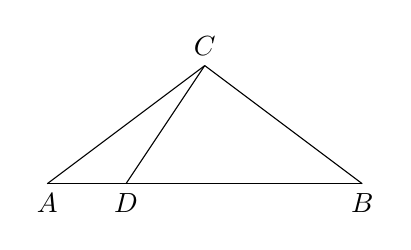
\begin{tikzpicture}
\coordinate [label=below:$A$](A) at (0,0);
\coordinate[label=below:$D$](D) at(1,0);
\coordinate[label=below:$B$](B) at(4,0);
\coordinate[label=above:$C$](C) at(2,1.5);
\foreach \p in{A,B,D}
\draw (C)--(\p);
\draw (A)--(B);
\end{tikzpicture}
\kongbai
\qs 已知函数$f(x)=\sin^2\left(x+\dfrac{\pi}{4}\right)$.
\begin{parts}
\part 求$f(x)$的最小正周期及其图象的对称轴方程;
\part 求$ f\left(\dfrac{\pi}{3}-x\right) $的单调递减区间.
\end{parts}
\end{questions}

\end{document}
